\documentclass[10pt,t]{beamer}
\usetheme{Heverlee}







% IDIOMA
\usepackage[utf8]{inputenc}
\usepackage[main=spanish]{babel}

% BIBLIOGRAFIA
\usepackage{natbib}
\usepackage{bibentry}

% INTERLINEADO DE PARRAFOS
\usepackage{setspace}
%\onehalfspacing

% Letras mayusculas
\usefonttheme{professionalfonts}

% Entornos
\theoremstyle{plain}
%\newtheorem{theorem}{Teorema}
\newtheorem{proposition}{Proposición}
\newtheorem{lema}{Lema}
%\newtheorem{corollary}{Corolario}

%\theoremstyle{definition}
%\newtheorem{definition}{Definición}
%\newtheorem{postulate}{Postulado}
%\newtheorem*{postulate 3'}{Postulate 3'}
%\newtheorem*{postulate 2'}{Projective Measurement}


\usepackage{times}

%\usepackage[latin1]{inputenc}

\usepackage{array}
\usepackage{amsmath}
\usepackage{amsthm}
\usepackage{amssymb}
\usepackage{graphicx}
\usepackage{hyperref}
\usepackage{longtable}
\usepackage{pdfpages}
\usepackage{eurosym} 
\usepackage{xcolor}

\usepackage[absolute,overlay]{textpos}
\usepackage{everypage}

\usepackage{pgf}
\usepackage{tikz}


\usepackage{setspace}  
\usepackage{colortbl}
\usepackage{graphicx}

\DeclareGraphicsExtensions{.jpg,.pdf,.mps,.png, svg}
\graphicspath{{../redaccion_tfg/figures/}{../redaccion_tfg/diagramas/}{../redaccion_tfg/wireframe/}}


%%% QUICK OPTIONS:
% (A) Math font without serifs, enable line below to make math serif:
    %\usefonttheme[onlymath]{serif}

% (B) Re-define primary colour by adjusting the RGB values
    %\definecolor{pblue}	{RGB}{206,125,66}

% (C) Title page graphic (optional) --- this is not for the background image, see \usebackgroundtemplate to change that ---
    %\titlegraphic{\includegraphics[height=2.7cm]{example_figure.pdf}}

% (D) Add logo to bottom right-corner (optional)
    %\logo{
\includegraphics[height=0.7cm]{logo.png}\hspace{12pt}\vspace{-6pt}}      

% (E) Choose one (or none) of these lines to add footline bar on all frames
    %\setbeamertemplate{footline}[infoline]  % author, title, insitute
    %\setbeamertemplate{footline}[navigation] % dots swhowing progress
    %\setbeamertemplate{footline}[navsym] % navigation symbols

% (F) Widescreen 16:9 ratio
    %\usepackage[orientation=landscape,size=custom,width=16,height=9,scale=0.45,debug]{beamerposter} 



%%% TITLE PAGE INFO:
\title[Modelos discretos en epidemiología]{Modelos discretos en epidemiología}
\subtitle{}
\author{Ana Buendía Ruiz-Azuaga}
\institute{Universidad de Granada}
\date{\today}

% Text inside {} is used on the title page. Text inside [] is optional, and is used in footline bar (if [] is omitted then text from {} will be used in both ; if [] is specified but left empty then the footline will not show any text)




 %%
 %%  0. TITLE PAGE and TABLE OF CONTENT
 %%
\begin{document}
% Title page

{
% Change image, or delete this line to remove background image
\usebackgroundtemplate{ \parbox[b][\paperheight][b]{\paperwidth}{\centering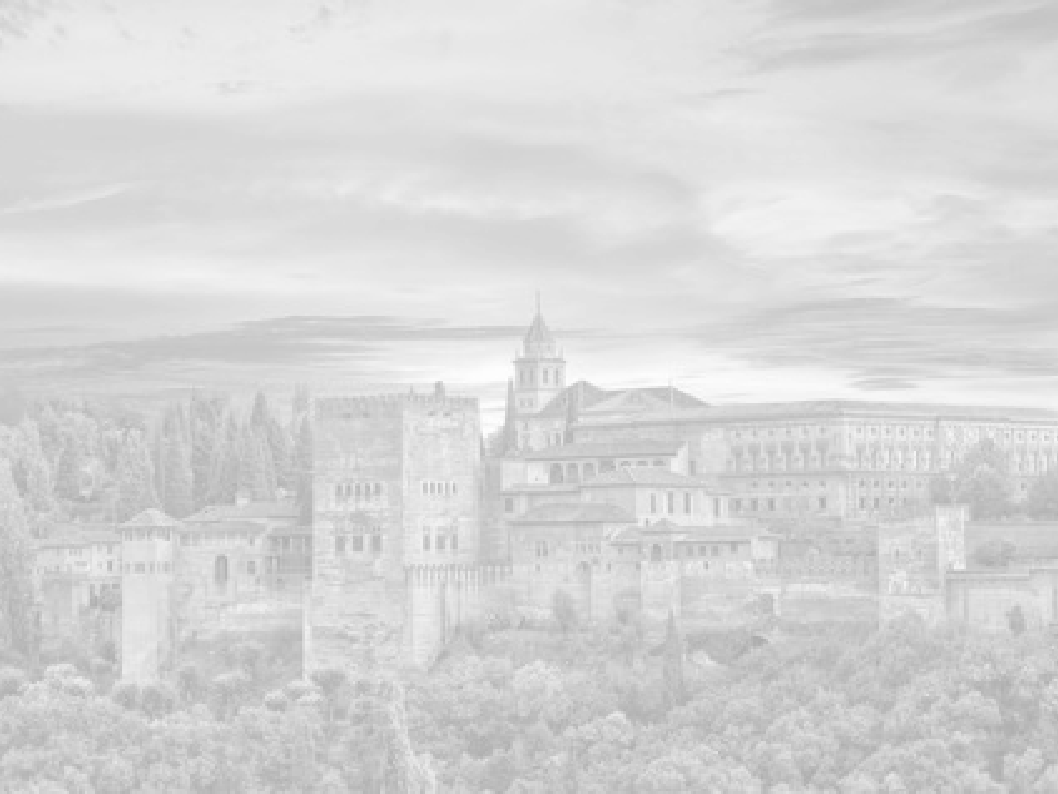
\includegraphics[width=\paperwidth]{Background/bg_alhambra.png}}} 
 %   abudhabi      cherry      forest      river
 %   alishan       chobe       leuven      sanfancisco
 %   blueprint     columns     library     uyuni
 %   bokeh         flowers     newyork     winter

%\setbeamercolor{background canvas}{bg=lgray}  % make background light gray

\begin{frame}[plain,noframenumbering]
    \titlepage
\end{frame}
}		


% Table of contents slide
\begin{frame}{Índice}
	\vskip 2mm
	\hfill	{\large \parbox{.95\textwidth}{\tableofcontents[hideothersubsections]}}
\end{frame}


\section{Introducción y objetivos}


\begin{frame}{Motivación}

\end{frame}


\begin{frame}{Objetivos}

\end{frame}


%%%%%%%%%%%%%%%%%%%%%%%%%%%%%%%%%%%%%%%%%%


\section{Herramientas básicas}


\begin{frame}{Conceptos clave}

\end{frame}


\begin{frame}{Ecuaciones en diferencias}

\end{frame}


\begin{frame}{Puntos fijos y estabilidad}

\end{frame}


\begin{frame}{Suposiciones base}

\end{frame}


%%%%%%%%%%%%%%%%%%%%%%%%%%%%%%%%%%%%%%%%%%


\section{Modelos discretos en epidemiología}


\subsection{Modelo SI}


\begin{frame}{Modelo SI}

\end{frame}


\subsection{Modelo SIS}


\begin{frame}{Modelo SIS}

\end{frame}


\subsection{Modelo SIR}


\begin{frame}{Modelo SIR}

\end{frame}


\subsection{Modelos multipoblacionales}


\begin{frame}{Modelos multipoblacionales}

\end{frame}


%%%%%%%%%%%%%%%%%%%%%%%%%%%%%%%%%%%%%%%%%%


\section{Modelos continuos en epidemiología}


\subsection{Modelo SI}


\begin{frame}{Modelo SI}

\end{frame}


\subsection{Modelo SIS}


\begin{frame}{Modelo SIS}

\end{frame}


\subsection{Modelo SIR}


\begin{frame}{Modelo SIR}

\end{frame}


%%%%%%%%%%%%%%%%%%%%%%%%%%%%%%%%%%%%%%%%%%


\section{Desarrollo del software: análisis y diseño}


\subsection{Análisis y diseño}


\begin{frame}{}

\end{frame}


\begin{frame}{Ajuste de datos}

\end{frame}


\subsection{Demostración}


\begin{frame}{Demostración de uso}

\end{frame}


\subsection{Datos reales}


\begin{frame}{El Covid-19 en España}

\end{frame}


\begin{frame}{El VIH en Baleares}

\end{frame}


%%%%%%%%%%%%%%%%%%%%%%%%%%%%%%%%%%%%%%%%%%


\section{Conclusiones}


\begin{frame}{Conclusiones}

\end{frame}


%%%%%%%%%%%%%%%%%%%%%%%%%%%%%%%%%%%%%%%%%%


\begin{frame}[c]{}
\begin{center}
\large{\textbf{Gracias por su atención.}}
\end{center}
\end{frame}



\end{document}